% f1992nl_q14_cube.tex — 1992 年·全国卷·理科 第 14 题（正方体与中点）
%
% 【来源】`.work/phase4-b15/source/1992全国理.pdf`（SHA-256 aa3c0a314b5ea0bf990cbc7d768575e3b3931da6ddbfb6c727681a516a7eb7aa），
%   第 1 页（印刷页 42）；内容流逐路径实测见 `.work/phase4-b15/transcripts/science-figures.md`。
%
% 【坐标口径】源 PDF 用户空间（原点左下、y 向上）。本图本地坐标
%   (x, y) = (x_page − 553.0000, y_page − 375.0000)，1 单位 = 1 TeX pt。
%   路径坐标逐点照录内容流（含三次贝塞尔控制点）。
%
% 元素计数：2 组路径（9 实＋3 虚＋AM/CN）＋10 个标签
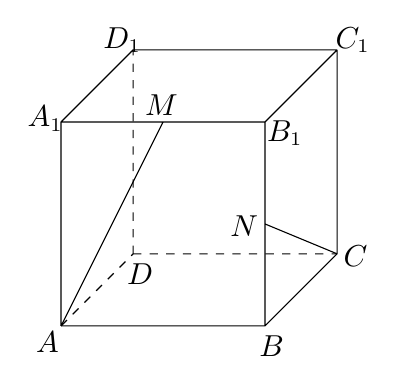
\begin{tikzpicture}[x=1pt, y=1pt,
    every node/.style={inner sep=0pt, font=\fontsize{10.5pt}{12.6pt}\selectfont}]
  \draw[line width=0.398pt] (5.6070,13.0830)   -- (79.3100,13.0830)   (79.3100,13.0830)   -- (105.3650,39.1370)   (79.3100,49.9350)   -- (105.3650,39.1370)   (5.6070,13.0830)   -- (42.4590,86.7860)   (5.6070,86.7860)   -- (79.3100,86.7860)   (79.3100,13.0830)   -- (79.3100,86.7860)   (5.6070,13.0830)   -- (5.6070,86.7860)   (105.3650,112.8410)   -- (79.3100,86.7860)   (105.3650,112.8410)   -- (31.6610,112.8410)   (5.6070,86.7860)   -- (31.6610,112.8410)   (5.6070,86.7860)   -- (5.6070,13.0830)   (79.3100,86.7860)   -- (79.3100,13.0830)   (105.3650,112.8410)   -- (105.3650,39.1370);
  \draw[line width=0.398pt, dash pattern=on 2.989pt off 2.989pt, dash phase=0.0pt] (5.6070,13.0830)   -- (31.6610,39.1370)   (31.6610,39.1370)   -- (105.3650,39.1370)   (31.6610,39.1370)   -- (31.6610,112.8410);

  \node[anchor=center] at (-0.100,88.000) {$A_1$};  % 源中心 (552.90,463.00)
  \node[anchor=center] at (86.500,82.700) {$B_1$};  % 源中心 (639.50,457.70)
  \node[anchor=center] at (111.000,116.300) {$C_1$};  % 源中心 (664.00,491.30)
  \node[anchor=center] at (27.700,116.300) {$D_1$};  % 源中心 (580.70,491.30)
  \node[anchor=center] at (0.700,7.200) {$A$};  % 源中心 (553.70,382.20)
  \node[anchor=center] at (81.700,5.700) {$B$};  % 源中心 (634.70,380.70)
  \node[anchor=center] at (112.000,38.200) {$C$};  % 源中心 (665.00,413.20)
  \node[anchor=center] at (34.200,31.700) {$D$};  % 源中心 (587.20,406.70)
  \node[anchor=center] at (41.900,92.800) {$M$};  % 源中心 (594.90,467.80)
  \node[anchor=center] at (71.800,49.000) {$N$};  % 源中心 (624.80,424.00)

\end{tikzpicture}
%
% 【自验结果】
%   探针：见 .work/phase4-b15/probe 的 verify_paths.py / check600_b15.py。
